\section{Versuchsaufbau/-durchführung}
Die Brennweite einer Linse wird im Versuch $V408$ auf drei
verschiedene Weisen bestimmt.
Die Verfahren werden im Folgenden kurz erklärt.

Als Lichtquelle wird eine Halogenlampe verwendet und als
Gegenstand ein \emph{Perl L}. Mit Hilfe eines Schirmes wird %Schirmes
das gebrochene Licht sichtbar gemacht werden.

\subsection{Untersuchung der Linsengleichung} %Versuchsteil sollte zur Überprüfung der Linsengleichung benutzt werden

Der Schirm, die Linse, das Perl L und die Lampe werden auf einer
Linie platziert.
Die Bildweite $b$ wird so lang verändert, bis ein scharfes Bild auf dem %man
Schirm zu erkennen ist. Das Wertepaar ($b$,$g$) werden notiert.
Danach wird die Position der Linse verändert und der Schirm neu eingestellt. %Satz
Es werden zehn Wertepaare notiert. %finde Prozess umständlich beschrieben
Mit Hilfe der Linsengleichung \eqref{eq: linsengleichung} und den Wertepaaren kann, dann die
Brennweite $f$ bestimmt werden. Der berechnetete Wert wird dann mit der bekannten Brennweite
verglichen, um so die Linsengleichung zu bestätigen.  %so war das nicht gedacht
Zusätzlich soll mit diesem Verfahren die Brennweite einer unbekannten Linse bestimmt werden.

\subsection{Bestimmung der Brennweite mit der Methode von Bessel}
Bei der Methode von Bessel wird die Entfernung zwischen %Satz
Gegenstand und Bild festgehalten. Die Linse wird so lang verschoben, bis zwei
Positionen gefunden worden sind, an denen ein scharfes Bild auf dem Schirm erkennbar ist.
Es ergeben sich folglich zwei Wertepaare ($b_1$,$g_1$) und ($b_2$,$g_2$).
Mit Hilfe der Hilfsgrößen $e=g_1+b_1=g_2+b_2$ und $d=g_1-b_1=g_2-b_2$ und der Formel %Formeln falsch
\begin{equation}
  \label{eq: bessel_methode}
  f=\frac{e^2-d^2}{4e}
\end{equation}
ist eine Berechnung der Brennweite möglich.
Nach der Aufnahme der Wertepaare wird die Linse neu positioniert.
Der Vorgang wird zehn Mal wiederholt.

Zusätzlich soll die chromatische Abberation der Linse untersucht werden,
dazu werden je fünf Wertepaare für rot und blau gefiltertes Filter
aufgenommen.
\subsection{Bestimmung der Brennweite mit der Methode von Abbe}
Die Methode von Abbe wird verwendet, um die Brennweite und die Lage der Hauptebenen
eines Linsensystems zu bestimmen. Hierzu wird der Abbildungsmaßstab $V$,
die Gegenstands- und Bildweite verwendet. Da die Hauptebenen nicht bekannt sind,
werden die Weiten $g'$ und $b'$ zu einem gewählten Punkt $A$ (vgl. Abb. \ref{fig: linsensystem}) gemessen.
Es gilt der Zusammenhang
\begin{align}
    g'=g+h=f\left(1+\frac{1}{V}\right)+h \label{eq: abstaende_abbe_g} \\
    b'=b+h'=f\left(1+V\right)+h' \label{eq: abstaende_abbe_b}.
\end{align}
Als Linsensystem werden eine Zerstreungs- und Sammellinse verwendet (vgl. Abbildung \ref{fig: linsensystem}). %Plural
\begin{figure}
    \centering
    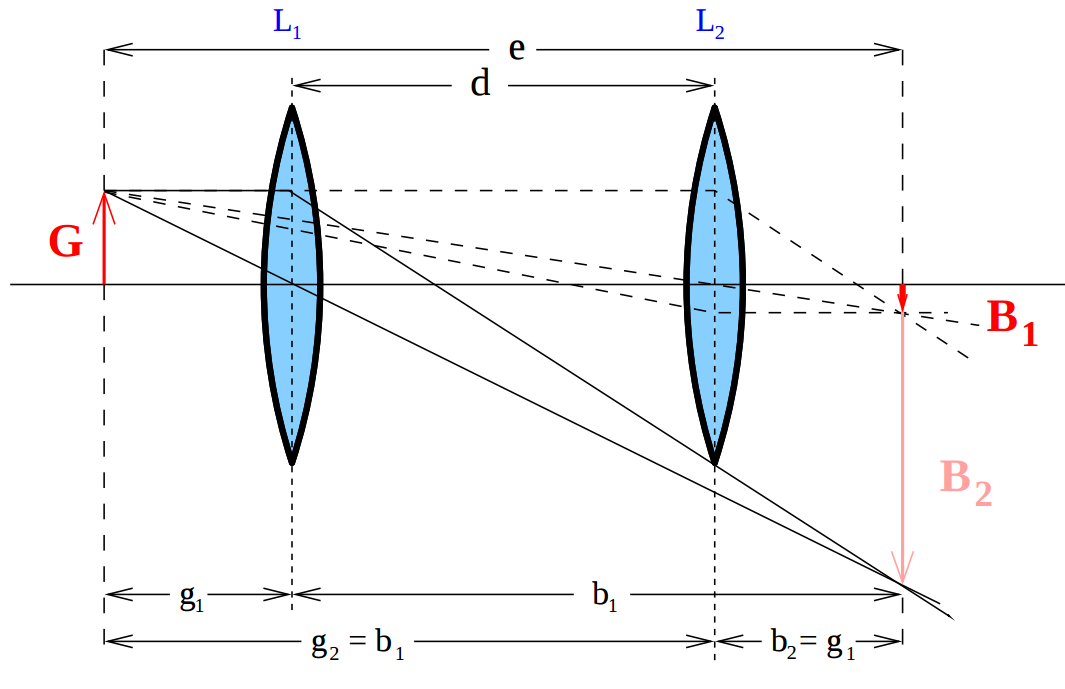
\includegraphics[width=0.6\textwidth]{./pics/linsensystem.png}
    \caption{Linsensystem \cite{anleitung408}.}
    \label{fig: linsensystem}
\end{figure}
Die relativen Bild- und Gegenstandsweiten werden von der Mittelebene
der Sammellinse gemessen.
Es wird der Schirm, bei fester Linsenposition, solang verschoben, bis ein scharfes
Bild auf dem Schirm erkennbar ist. Nun werden $g'$, $b'$ und $B$ notiert.
Mit Hilfe von \eqref{eq: abbildungsgesetz_gross} bzw. \eqref{eq: abbildungsgesetz_klein}
kann $V$ bestimmt werden.
Für zehn verschiedene Linsenpositionen werden die Werte aufgeschrieben. %kein Komma
